% =====================================================================
%  Лекция 2. УЗБЧ в форме Колмогорова. Теорема Гливенко--Кантелли.
%  Дата: 2026-09-24
% =====================================================================
% В квадратных скобках — короткое название для оглавления и закладок PDF.
\section[Эмпирическая вероятность. УЗБЧ. Теорема Гливенко--Кантелли]%
  {Теорема о~предельном распределении эмпирической вероятности.
   Усиленный закон больших чисел в~форме Колмогорова.
   Теорема Гливенко--Кантелли}
\label{lec:02}

\subsection{Теорема о предельном распределении эмпирической вероятности}

\begin{reminder}
  Последовательность случайных величин $\{\xi_n, n \in \N\}$ сходится
  к случайной величине~$\xi$ почти наверное, если
  \[
    \P\Bigl(\bigl\{\omega \colon \lim_{n \to \infty} \xi_n(\omega) = \xi(\omega)\bigr\}\Bigr) = 1.
  \]
  Обозначение: $\xi_n \toas \xi$.
\end{reminder}

\begin{theorem}[УЗБЧ Колмогорова]
  \label{lec02:slln}
  Пусть $\{\xi_n, n \in \N\}$~--- последовательность независимых
  одинаково распределённых случайных величин, причём $\E\abs{\xi_1} < \infty$. Тогда
  \[
    \frac{\xi_1 + \cdots + \xi_n}{n} \toas a = \E\xi_1 \quad \textup{при } n \to \infty.
  \]
\end{theorem}

Теорема принимается без доказательства.

\begin{theorem}
  \label{lec02:emp-prob}
  Для любого $B \in \mathcal{B}(\R)$ выполняется
  \[
    \Pemp(B) \toas \P_\xi(B) \quad \textup{при } n \to \infty,
  \]
  и для любого $x \in \R$ выполняется
  \[
    F_n^*(x) \toas F_\xi(x) \quad \textup{при } n \to \infty.
  \]
\end{theorem}

\begin{proof}
  По определению эмпирической вероятности
  \[
    \Pemp(B) = \frac{1}{n} \sum_{k=1}^{n} \Ind{X_k \in B},
  \]
  то есть $\Pemp(B)$~--- выборочное среднее индикаторов $\Ind{X_k \in B}$.
  Индикаторы независимы и одинаково распределены, поскольку такими являются~$X_k$, и
  \[
    \E\Ind{X_k \in B} = \P\{X_k \in B\} = \P_\xi(B).
  \]
  Индикаторы ограничены, поэтому $\E\abs{\Ind{X_k \in B}} \le 1 < \infty$, и по
  УЗБЧ в форме Колмогорова (\cref{lec02:slln}) получаем
  \[
    \Pemp(B) = \frac{1}{n} \sum_{k=1}^{n} \Ind{X_k \in B} \toas \P_\xi(B)
    \quad \textup{при } n \to \infty.
  \]
  Второе утверждение получается из первого при $B = (-\infty, x]$:
  $F_n^*(x) = \Pemp\bigl((-\infty, x]\bigr)$ и $F_\xi(x) = \P_\xi\bigl((-\infty, x]\bigr)$.
\end{proof}

\subsection{Теорема Гливенко--Кантелли}

\begin{theorem}[Гливенко--Кантелли]
  \label{lec02:glivenko}
  Пусть $F_\xi(x)$~--- функция распределения случайной величины~$\xi$,
  а $F_n^*(x)$~--- эмпирическая функция распределения, построенная по выборке из~$\xi$. Тогда
  \[
    \sup_{x \in \R} \abs{F_n^*(x) - F_\xi(x)} \toas 0 \quad \textup{при } n \to \infty.
  \]
\end{theorem}

\begin{remark}
  Не помню доказывали ли это на лекции, но пусть доказательство будет (если что, его писал клод, я сам в это доказательство особо не вникал).
\end{remark}

\paragraph{Идея.} По теореме~\ref{lec02:emp-prob} для каждого фиксированного~$x$
выполнено $F_n^*(x) \toas F_\xi(x)$, то есть сходимость имеет место на своём событии
вероятности~1 для каждого~$x$. Но точек~$x$ несчётно много, и пересечь все эти события
нельзя. Поэтому сводим задачу к \emph{конечному} числу точек: обе функции $F_n^*$
и $F_\xi$ не убывают, и если они близки в узлах достаточно мелкой сетки, то близки
и между узлами.

Всюду ниже $F = F_\xi$, и полагаем $F(-\infty) = F_n^*(-\infty) = 0$,
$F(+\infty) = F_n^*(+\infty) = 1$.

\begin{figure}[h]
  \centering
  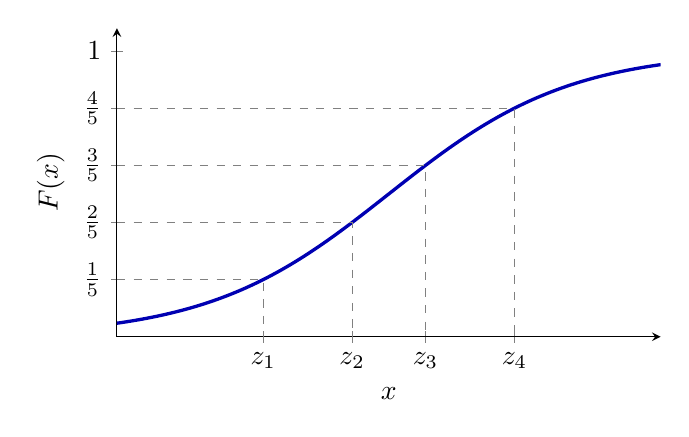
\begin{tikzpicture}
    \begin{axis}[
      width=0.7\textwidth, height=5.5cm,
      xmin=0, xmax=6, ymin=0, ymax=1.08,
      axis lines=left, xlabel={$x$}, ylabel={$F(x)$},
      xtick={1.614, 2.595, 3.405, 4.386},
      xticklabels={$z_1$, $z_2$, $z_3$, $z_4$},
      ytick={0.2, 0.4, 0.6, 0.8, 1},
      yticklabels={$\frac15$, $\frac25$, $\frac35$, $\frac45$, $1$},
    ]
      \addplot[very thick, blue!70!black, domain=0:6, samples=120] {1/(1 + exp(-(x - 3)))};
      \addplot[dashed, gray] coordinates {(0, 0.2) (1.614, 0.2) (1.614, 0)};
      \addplot[dashed, gray] coordinates {(0, 0.4) (2.595, 0.4) (2.595, 0)};
      \addplot[dashed, gray] coordinates {(0, 0.6) (3.405, 0.6) (3.405, 0)};
      \addplot[dashed, gray] coordinates {(0, 0.8) (4.386, 0.8) (4.386, 0)};
    \end{axis}
  \end{tikzpicture}
  \caption{Сетка из случая~1 при $r = 5$: уровни $\frac{k}{r}$ на оси ординат
           дают узлы $z_k$, и между соседними узлами $F$ растёт ровно на $\frac1r < \varepsilon$.}
  \label{lec02:fig:grid}
\end{figure}

\begin{proof}
  \emph{Случай 1: $F$ непрерывна на~$\R$.}

  \emph{Шаг 1: сетка.} Зафиксируем $\varepsilon > 0$ и выберем $r \in \N$ так, что
  $\frac1r < \varepsilon$. Так как $F$ непрерывна и меняется от~0 до~1, по теореме
  о промежуточном значении для каждого $k = 1, \ldots, r - 1$ найдётся точка~$z_k$
  с $F(z_k) = \frac{k}{r}$ (см.~\cref{lec02:fig:grid}). Положим $z_0 = -\infty$,
  $z_r = +\infty$. Получаем сетку
  \[
    -\infty = z_0 < z_1 < \ldots < z_r = +\infty, \qquad
    F(z_{k+1}) - F(z_k) = \frac1r < \varepsilon.
  \]

  \emph{Шаг 2: событие вероятности~1.} Пусть
  $A_k = \{F_n^*(z_k) \to F(z_k)\}$, $k = 1, \ldots, r - 1$. По теореме~\ref{lec02:emp-prob}
  $\P(A_k) = 1$. Положим $A(\varepsilon) = A_1 \cap \ldots \cap A_{r-1}$. Событий конечное
  число, поэтому
  $\P\bigl(\overline{A(\varepsilon)}\bigr) \le \sum_{k=1}^{r-1} \P(\overline{A_k}) = 0$,
  то есть $\P\bigl(A(\varepsilon)\bigr) = 1$. В крайних узлах $z_0, z_r$ сходимость
  не нужна: там $F_n^*$ и $F$ просто равны.

  \emph{Шаг 3: близость в узлах.} Зафиксируем $\omega \in A(\varepsilon)$. Узлов
  конечное число, поэтому найдётся $n_0 = n_0(\omega, \varepsilon)$ такой, что при всех
  $n \ge n_0$ сразу для всех $k = 0, \ldots, r$
  \[
    \abs{F_n^*(z_k) - F(z_k)} < \varepsilon.
  \]

  \emph{Шаг 4: оценка между узлами.} Возьмём любое $x \in \R$; оно попадает в
  некоторый промежуток $z_k \le x < z_{k+1}$. Обе функции не убывают, поэтому
  $F_n^*(z_k) \le F_n^*(x) \le F_n^*(z_{k+1})$ и $F(z_k) \le F(x) \le F(z_{k+1})$.
  Отсюда при $n \ge n_0$
  \begin{align*}
    F_n^*(x) - F(x) &\le F_n^*(z_{k+1}) - F(z_k)
      = \bigl(F_n^*(z_{k+1}) - F(z_{k+1})\bigr) + \bigl(F(z_{k+1}) - F(z_k)\bigr)
      < 2\varepsilon, \\
    F_n^*(x) - F(x) &\ge F_n^*(z_k) - F(z_{k+1})
      = \bigl(F_n^*(z_k) - F(z_k)\bigr) - \bigl(F(z_{k+1}) - F(z_k)\bigr)
      > -2\varepsilon.
  \end{align*}
  (В верхней оценке $F_n^*$ берём в правом узле, а $F$~--- в левом; в нижней наоборот.)
  Значит, $\abs{F_n^*(x) - F(x)} < 2\varepsilon$ для всех $x$ одновременно, то есть на
  $A(\varepsilon)$
  \[
    \sup_{x \in \R} \abs{F_n^*(x) - F(x)} \le 2\varepsilon \quad \text{при } n \ge n_0.
  \]

  \emph{Шаг 5: $\varepsilon \to 0$.} Сетка, а значит и событие $A(\varepsilon)$, зависит
  от~$\varepsilon$. Возьмём $\varepsilon = \frac1m$, $m \in \N$, и положим
  $A^* = \bigcap_{m=1}^{\infty} A\bigl(\tfrac1m\bigr)$. Пересечение счётное, поэтому
  $\P(A^*) = 1$. При $\omega \in A^*$ для любого~$m$
  \[
    \limsup_{n \to \infty} \sup_{x \in \R} \abs{F_n^*(x) - F(x)} \le \frac2m,
  \]
  значит, этот верхний предел равен нулю, то есть
  $\sup_{x} \abs{F_n^*(x) - F(x)} \to 0$ на~$A^*$. Так как $\P(A^*) = 1$, это и есть
  сходимость почти наверное.

  \medskip
  \emph{Случай 2: $F$ может иметь разрывы.} Если у $F$ есть скачок больше~$\varepsilon$,
  сетку из шага~1 построить нельзя: на промежутке, содержащем этот скачок,
  $F$ вырастет больше чем на~$\varepsilon$. Поэтому скачки ставим в узлы, а в правом
  узле берём левый предел $F(z - 0)$. Меняются шаги~1--4, шаг~5 тот же.

  \emph{Шаг 1: сетка.} Нужна сетка $-\infty = z_0 < z_1 < \ldots < z_r = +\infty$ с
  \[
    F(z_{k+1} - 0) - F(z_k) < \varepsilon, \qquad k = 0, \ldots, r - 1.
  \]
  Строим её по шагам: при уже выбранном $z_k$ положим
  \[
    z_{k+1} = \inf\bigl\{z > z_k : F(z) \ge F(z_k) + \tfrac{\varepsilon}{2}\bigr\}
  \]
  (если множество пусто, $z_{k+1} = +\infty$, и построение закончено). При $z_k < z < z_{k+1}$
  выполнено $F(z) < F(z_k) + \frac\varepsilon2$, откуда
  $F(z_{k+1} - 0) - F(z_k) \le \frac\varepsilon2 < \varepsilon$. С другой стороны, $F$
  непрерывна справа, поэтому $F(z_{k+1}) \ge F(z_k) + \frac\varepsilon2$: на каждом шаге
  $F$ увеличивается хотя бы на $\frac\varepsilon2$, и шагов не больше $\frac2\varepsilon$.
  Значит, сетка конечна.

  Все скачки больше $\frac\varepsilon2$ автоматически оказываются узлами сетки~--- в
  учебнике это делается явно: такие точки разрыва (их не больше $\frac2\varepsilon$)
  сразу включают в сетку.

  \emph{Шаг 2: событие.} Кроме $A_k$ нужны события
  $A_k^- = \{F_n^*(z_k - 0) \to F(z_k - 0)\}$. Так как
  $F(z - 0) = \P_\xi\bigl((-\infty, z)\bigr)$ и $F_n^*(z - 0) = \Pemp\bigl((-\infty, z)\bigr)$,
  по теореме~\ref{lec02:emp-prob} с $B = (-\infty, z_k)$ получаем $\P(A_k^-) = 1$. Положим
  $A(\varepsilon) = \bigcap_{k=1}^{r-1} (A_k \cap A_k^-)$; событий по-прежнему конечное
  число, и $\P\bigl(A(\varepsilon)\bigr) = 1$.

  \emph{Шаг 3.} Как в случае~1, но при $n \ge n_0$ близки и значения, и левые пределы:
  $\abs{F_n^*(z_k) - F(z_k)} < \varepsilon$ и
  $\abs{F_n^*(z_k - 0) - F(z_k - 0)} < \varepsilon$ для всех~$k$.

  \emph{Шаг 4.} При $z_k \le x < z_{k+1}$ из монотонности
  $F_n^*(z_k) \le F_n^*(x) \le F_n^*(z_{k+1} - 0)$ и
  $F(z_k) \le F(x) \le F(z_{k+1} - 0)$, поэтому
  \begin{align*}
    F_n^*(x) - F(x) &\le F_n^*(z_{k+1} - 0) - F(z_k) \\
      &= \bigl(F_n^*(z_{k+1} - 0) - F(z_{k+1} - 0)\bigr)
        + \bigl(F(z_{k+1} - 0) - F(z_k)\bigr) < 2\varepsilon, \\
    F_n^*(x) - F(x) &\ge F_n^*(z_k) - F(z_{k+1} - 0) \\
      &= \bigl(F_n^*(z_k) - F(z_k)\bigr) - \bigl(F(z_{k+1} - 0) - F(z_k)\bigr) > -2\varepsilon.
  \end{align*}
  Дальше~--- дословно шаг~5 случая~1.
\end{proof}

\begin{remark}
  Случай~1~--- частный случай случая~2: если $F$ непрерывна, то $F(z - 0) = F(z)$.
  Отдельно он разобран, потому что в нём проще увидеть идею.
\end{remark}


\begin{reminder}[Сходимость по распределению]
  Последовательность случайных величин $\{\xi_n, n \in \N\}$ сходится
  к случайной величине~$\xi$ по распределению, если в каждой точке~$x$,
  в которой $F_\xi$ непрерывна, выполнено
  \[
    F_{\xi_n}(x) \to F_\xi(x) \quad \text{при } n \to \infty.
  \]
  Обозначение: $\xi_n \tod \xi$.
\end{reminder}

\begin{theorem}
  \label{lec02:clt-emp}
  Для любого борелевского множества $B \in \mathcal{B}(\R)$ выполняется
  \[
    \sqrt{n}\bigl(\Pemp(B) - \P_\xi(B)\bigr) \tod \zeta \sqrt{\P_\xi(B)\bigl(1 - \P_\xi(B)\bigr)}
    \quad \textup{при } n \to \infty,
  \]
  где $\zeta \sim \Norm(0, 1)$.
\end{theorem}

\begin{proof}
  Обозначим $p = \P_\xi(B)$. По определению эмпирической вероятности
  \[
    \Pemp(B) - p = \frac{1}{n} \sum_{k=1}^{n} \bigl(\Ind{X_k \in B} - p\bigr).
  \]
  Индикаторы $\Ind{X_k \in B}$ независимы, одинаково распределены и имеют
  распределение $\Bern(p)$, поэтому
  \[
    \E\Ind{X_k \in B} = p, \qquad \D\Ind{X_k \in B} = p(1 - p).
  \]
  Применяя ЦПТ для независимых одинаково распределённых случайных величин, получаем
  \[
    \sqrt{n}\bigl(\Pemp(B) - p\bigr)
    = \frac{\sum_{k=1}^{n} \bigl(\Ind{X_k \in B} - p\bigr)}{\sqrt{n}}
    \tod \zeta \sqrt{p(1 - p)}. \qedhere
  \]
\end{proof}
